% \RequirePackage[l2tabu, orthodox]{nag} % 检测已被淘汰的宏包及过时的命令
\documentclass[twocolumn]{IEEEtran}

%%%%%%%%%%%% official suggested packages  %%%%%%%%%%%%
% \usepackage{cite} % 用 natbib 代替
\usepackage[pdftex]{graphicx} % 插图命令 \includegraphics
\usepackage{amsmath} % Math Packages
% 模板要求不许使用 algorithm.sty 和 algorithm2e.sty
% 模板允许使用 algorithmicx.sty
\usepackage{algorithmic}
\usepackage{array} % Alignment Packages
% 模板要求必须开启 caption=false
\usepackage[caption=false,font=footnotesize]{subfig} % Subfigure Packages
% 模板要求不许使用 cuted.sty 和 midfloat.sty
% Float Packages
% 原先用 dblfloatfix，但它内部 \RequirePackage{fixltx2e}，而 fixltx2e 的修正
% 自 LaTeX 2015 起已并入内核，只会输出一条无用警告。
% stfloats 单独提供 dblfloatfix 的全部能力（跨栏浮动体可置底，\@dbflt 默认 [tbp]），
% 且仍在维护。注意：stfloats 与 dblfloatfix 互斥，不可同时载入。
\usepackage{stfloats}
\usepackage{url} % simple URL typesetting

%%%%%%%%%%%% packages added by myself %%%%%%%%%%%%
% 调整单词、字母的间距，需要放在字体宏包之前
\usepackage{microtype}
\usepackage[utf8]{inputenc} % allow utf-8 input
\usepackage[T1]{fontenc}    % use 8-bit T1 fonts
% \usepackage{booktabs}       % professional-quality tables，也就是三线表
\usepackage{paralist} % Compacted versions of enumerate and itemize.
\usepackage{marvosym} % 常用符号, 特别是打勾、打叉
\usepackage{bm} % 实现字体的斜体加粗
\usepackage{bbm} % fix \mathbb doesn't support digits
% \usepackage{amsfonts}  % for \mathbb, blackboard bold，黑板粗体
\usepackage{amssymb}   % 黑板粗体 \mathbb, 德文尖角体 \mathfrak, \backsim
\usepackage{mathrsfs} % 花体 \mathscr
\usepackage{tabularray} % tblr or talltblr or longtblr environment
\UseTblrLibrary{booktabs}       % professional-quality tables，也就是三线表
\usepackage{tabularx} % 自动计算列宽的表格包
\usepackage[flushleft]{threeparttable} % 给表格项添加注释
\usepackage{colortbl} % 表格行列颜色
\usepackage{makecell} % 表格内容换行
\usepackage{multirow} % 多行表格
\usepackage{nicefrac} % 斜着的分号
\usepackage[dvipsnames]{xcolor} % 字体颜色
\usepackage{soul} % highlight, strikeout, underline
\setul{0.5ex}{0.3ex}
\newcommand{\ulcolor}[2][Red]{\setulcolor{#1}\ul{#2}}
% Extensive support for hypertext, in order to cross-reference.
% \usepackage[bookmarks=false,breaklinks=true,colorlinks=true,
%             linkcolor=red,pagebackref=true]{hyperref}
% \usepackage{hyperref}
% \hypersetup{
%     colorlinks=true,
%     linkcolor=blue,
%     filecolor=magenta,
%     urlcolor=cyan}
% \definecolor{citecolor}{RGB}{34,139,34}
\definecolor{citecolor}{RGB}{0,0,255}
% \usepackage[pagebackref=true,breaklinks=true,letterpaper=true,colorlinks,
%     citecolor=citecolor,bookmarks=false]{hyperref}
% letterpaper 选项已被新版 hyperref 废弃（纸张尺寸由 IEEEtran 决定），故移除
\usepackage[pagebackref=false,breaklinks=true,colorlinks,
    citecolor=citecolor,bookmarks=false]{hyperref}
\usepackage{cleveref}  % for \cref
\crefformat{figure}{Fig.~#2#1#3}
\crefformat{equation}{Eq.~(#2#1#3)}
\crefformat{table}{Table~#2#1#3}
\crefformat{section}{Section~#2#1#3}
\crefformat{algorithm}{Algorithm~#2#1#3}
\crefformat{appendix}{Appendix #2#1#3}
\crefformat{subsection}{subsection~#2#1#3}
\usepackage{cellspace}
\usepackage[numbers,sort&compress]{natbib} % 代替 cite.sty
\renewcommand{\bibfont}{\small}
\usepackage{xspace} % 用于在 \newcommand 中添加空格
\newcommand{\ie}{i.\nolinebreak[4]\hspace{0.01em}\nolinebreak[4]e.\@\xspace}
\newcommand{\eg}{e.\nolinebreak[4]\hspace{0.01em}\nolinebreak[4]g.\@\xspace}
\newcommand{\etal}{\emph{et al.}\xspace}

\usepackage{pifont} % http://ctan.org/pkg/pifont
\newcommand{\cmark}{\ding{51}}%
\newcommand{\xmark}{\ding{53}}%
% \newcommand{\red}[1]{\textcolor{red}{#1}}
% \newcommand{\blue}[1]{\textcolor{blue}{#1}}
% \newcommand{\todo}{\red{[TODO]~}}
% \newcommand{\todot}[1]{\red{[TODO]~#1~}}

\newcommand{\rewrite}[1]{{\textcolor{red}{#1}}} % 重写

% Table Column Color
\newcommand{\mc}[2]{\multicolumn{#1}{c}{#2}}
\definecolor{Gray}{rgb}{0.9,0.9,0.9}
\definecolor{LightCyan}{rgb}{0.88,1,1}
% 自定义带底色的居中列。注意 b 是 array 的原生列类型（底对齐 parbox，用法 b{3cm}），
% 不能占用，否则 array 会报 "Redefining primitive column b"，且原生用法失效。
% 这里白底列改用 n（none/normal），array 原生的 c l r m b p 均保持原义。
\newcolumntype{a}{>{\columncolor{Gray}}c} % 灰底居中列
\newcolumntype{n}{>{\columncolor{white}}c} % 白底居中列（原名 b，已改名）

\begin{document}

\setlength{\abovedisplayskip}{.5\baselineskip} % 调整公式与正文间的段前距离
\setlength{\belowdisplayskip}{.5\baselineskip} % 调整公式与正文间的段后距离


\title{Motion-Adaptive Long-Term Memory Network for Fast-Moving Infrared Small Target Detection}


% author names and IEEE memberships
% !TEX root = ../main.tex

% author names and IEEE memberships
\author{
    Ruimin Huang,
    Jun Huang,
    Yong Ma,
    Fan Fan,
    and Yiming Zhu

    \thanks{
        % This work was supported in part by the National Natural Science Foundation of China under Grant 62475199, Grant 62473297, and Grant U23B2050. \emph{(Corresponding author: Fan Fan.)}
        This work was supported in part by the National Natural Science Foundation of China under Grants 62473297, 62475199, and U23B2050, and in part by the National Key R\&D Program of China under Grant 2024YFE0202500. \emph{(Corresponding author: Fan Fan.)}
    }

    \thanks{
        Ruimin Huang and Yiming Zhu are with the Electronic Information School, Wuhan University, Wuhan 430072, China
        (e-mail: \href{mailto:huang_ruimin@whu.edu.cn}{huang\_ruimin@whu.edu.cn}; 
        \href{mailto:yiming_zhu_2015@163.com}{yiming\_zhu\_2015@163.com}).

        Jun Huang, Yong Ma, and Fan Fan are with the School of Robotics, Wuhan University, Wuhan 430072, China
        (e-mail: \href{mailto:junhwong@whu.edu.cn}{junhwong@whu.edu.cn};
        \href{mailto:mayong@whu.edu.cn}{mayong@whu.edu.cn};
        \href{mailto:fanfan@whu.edu.cn}{fanfan@whu.edu.cn}).
    }
}


\maketitle

% !TEX root = ../main.tex

\begin{abstract}
The code is available at \url{https:}.
\end{abstract}

\begin{IEEEkeywords}
Infrared small target, semantic segmentation, attention mechanism, feature selection, feature fusion.
\end{IEEEkeywords}
\vspace{-1\baselineskip}

% !TEX root = ../main.tex
% \bibliography{../reference.bib}


\section{Introduction} \label{sec:introduction}


To start \cite{sobrino2016review}
% !TEX root = ../main.tex
% \bibliography{../reference.bib}

\section{Related Work} \label{sec:Related Work}


% !TEX root = ../main.tex
% \bibliography{../reference.bib}

\section{Method} \label{sec:method}

% !TEX root = ../main.tex
% \bibliography{../reference.bib}



\section{Experiments and Analysis} \label{sec:experiment}

% !TEX root = ../main.tex

\section{Conclusion} \label{sec:conclusion}


\bibliographystyle{IEEEtran}
\bibliography{./reference.bib}

% !TEX root = ../main.tex

% Ruimin Huang
\begin{IEEEbiography}[{
\includegraphics[width=1.1in,height=1.35in,clip,keepaspectratio]{./figs/biography/Ruimin_Huang}}]{Ruimin Huang} received the M.S. degree in optical engineering from the School of Physics and Electronic Information, Yunnan Normal University, Kunming, China, in 2024. He is currently pursuing the Ph.D. degree in electronic information with the Electronic Information School, Wuhan University, Wuhan, China.

His research interests include computer vision, infrared technology, and remote sensing.
\end{IEEEbiography}

% Jun Huang
\begin{IEEEbiography}[{
\includegraphics[width=1.1in,height=1.35in,clip,keepaspectratio]{./figs/biography/Jun_Huang}}]{Jun Huang} (Member, IEEE) received the B.S. degree in communication engineering and the Ph.D. degree in electronic circuit and system from the Huazhong University of Science and Technology, Wuhan, China, in 2008 and 2014, respectively.

He is currently a Professor with the School of Robotics, Wuhan University, Wuhan. His main research interests include infrared image and infrared spectrum processing.
\end{IEEEbiography}

% Yong Ma
\begin{IEEEbiography}[{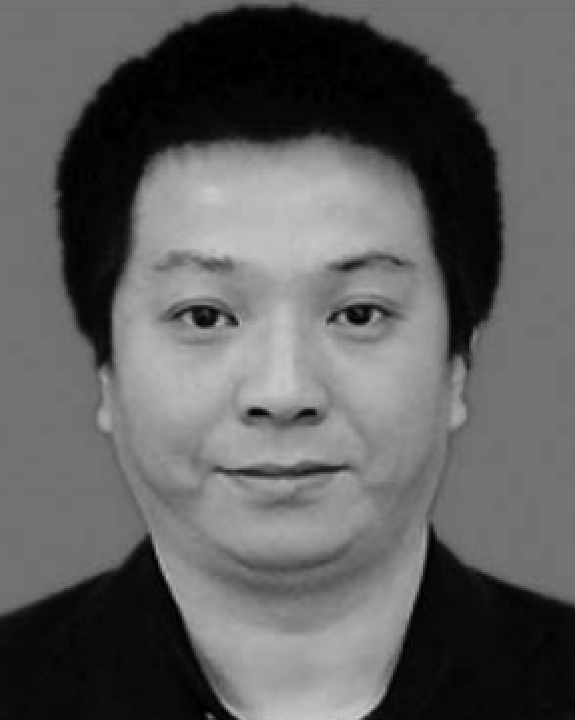
\includegraphics[width=1.0in,height=1.34in,clip,keepaspectratio]{./figs/biography/Yong_Ma}}]{Yong Ma} received the B.S. degree in industrial automation and the M.S. degree in automatic control from the Beijing Institute of Technology, Beijing, China, in 1994 and 1997, respectively, and the Ph.D. degree in electronic circuit and system from the Huazhong University of Science and Technology (HUST), Wuhan, China, in 2003.

From 2004 to 2006, he was a Lecturer with the University of the West of England, Bristol, U.K. From 2006 to 2014, he was a Professor of electronics with Wuhan National Laboratory for Optoelectronics, HUST. He is currently a Professor with the School of Robotics, Wuhan University, Wuhan. His research interests include signal and systems, infrared image processing, pattern recognition, and interface circuits to sensors and actuators.
\end{IEEEbiography}

% Fan Fan
\begin{IEEEbiography}[{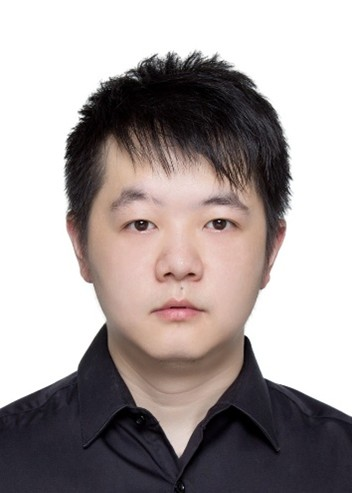
\includegraphics[width=1.1in,height=1.35in,clip,keepaspectratio]{./figs/biography/Fan_Fan}}]{Fan Fan} (Member, IEEE) received the B.S. degree in communication engineering and the Ph.D. degree in electronic circuit and system from the Huazhong University of Science and Technology, Wuhan, China, in 2009 and 2015, respectively.

He is currently an Associate Professor with the School of Robotics, Wuhan University, Wuhan. His research interests include infrared thermal imaging, machine learning, and computer vision.
\end{IEEEbiography}

% Yiming Zhu
\begin{IEEEbiography}[{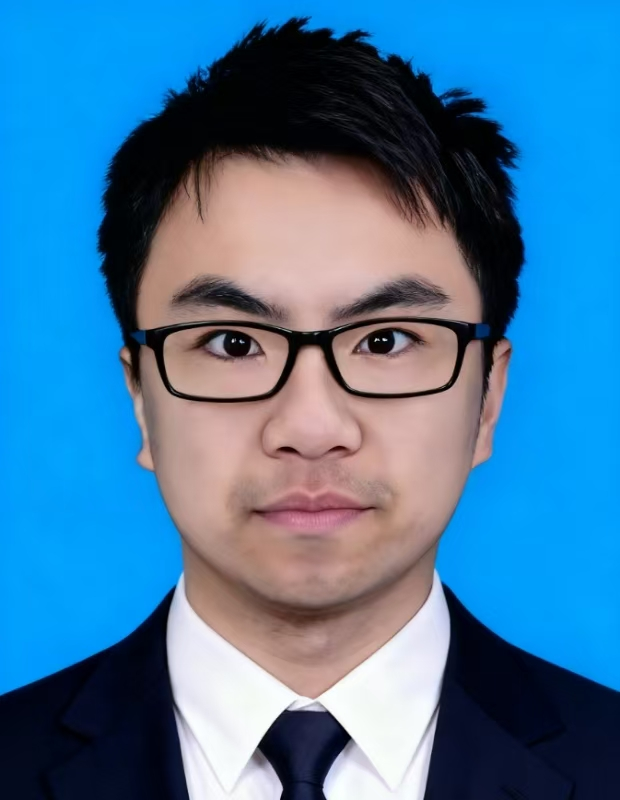
\includegraphics[width=1.0in,height=1.35in,clip,keepaspectratio]{./figs/biography/Yiming_Zhu}}]{Yiming Zhu} received the M.S. degree in optical engineering from the School of Optics and Photonics, Beijing Institute of Technology (BIT), Beijing, China, in 2022. He is currently pursuing the Ph.D. degree with the Multi-Spectral Vision Processing (MVP) Lab, Electronic Information School, Wuhan University, Wuhan, China.

His research interests include computer vision, infrared technology, and remote sensing.
\end{IEEEbiography}
 % 作者介绍

\end{document}
